\documentclass{beamer}
\usepackage[utf8]{inputenc}
\usepackage{graphicx}
\usepackage{url}
\usepackage{cite}
\usepackage[table]{xcolor}
\usepackage{tikz}
\usetikzlibrary{positioning}

% Professional font setup for presentations
\usepackage[T1]{fontenc}
\usepackage{helvet}  % Clean sans-serif font for presentations
\renewcommand{\familydefault}{\sfdefault}  % Use Helvetica as default

\usetheme{Madrid}
\usecolortheme{default}

\title{Dynamic IoT Applications and Isomorphic IoT Systems Using WebAssembly}
\subtitle{A Case Study Analysis}
\author{Uddhav P. Gautam \& Ram Mude}
\institute{ECE 4984/5984 IoT System Design\\Virginia Tech}
\date{}

\begin{document}

% Title slide
\begin{frame}
\titlepage
\end{frame}

% Slide 2: Problem Statement
\begin{frame}
\frametitle{Problem Statement}
\framesubtitle{Critical Challenges in Modern IoT Development}

\textbf{Challenge 1: Slow Device Updates}
\begin{itemize}
\item Traditional firmware updates require 10+ seconds downtime
\item Full system reboot needed for every update
\item Cannot respond quickly to changing user requirements (ML model updates, sensor calibration changes)
\end{itemize}

\textbf{Challenge 2: Multi-Platform Complexity}
\begin{itemize}
\item IoT systems span device, edge, and cloud layers (Raspberry Pi, Google Cloud, local machine)
\item Different platforms require different technologies (ARM, x86/64, different OS)
\item Multiple codebases increase maintenance burden (separate implementations for ARM, x86/64, arm64)
\end{itemize}

\textbf{Research Question:} How can WebAssembly solve these IoT development challenges?
\end{frame}

% Slide 3: Proposed Solutions
\begin{frame}
    \frametitle{Proposed Solutions}
    \framesubtitle{Two Innovative WebAssembly-Based Approaches}
    
    \textbf{Solution 1: Dynamic IoT Applications}
    \begin{itemize}
    \item Partial updates without system reboot
    \item Only restart Wasm runtime (1.4s vs 10s+)
    \item Enable rapid response to user requirements (ML model updates, bug fixes)
    \end{itemize}
    
    \textbf{Solution 2: Isomorphic IoT Systems}
    \begin{itemize}
    \item Same Wasm binary across all layers (device, edge, cloud)
    \item Common codebase for device, edge, cloud (single Rust/Elixir codebase)
    \item Improved development efficiency and maintainability (common codebase across platforms)
    \end{itemize}
    
    \textbf{Key Innovation:} WebAssembly's platform-agnostic execution enables both solutions
    \end{frame}


% Slide 4: Isomorphic Architecture with Wasmtube Bridge
\begin{frame}
    \frametitle{Same Wasm Binary Runs Across All Layers!}
    \framesubtitle{Wasmtube Bridge Enables Dynamic Updates}
    
    \begin{center}
    \small
    \begin{tabular}{|p{2.5cm}|p{2.5cm}|p{2.5cm}|p{2.5cm}|}
    \hline
    \multicolumn{4}{|c|}{\textbf{Wasm Runtime}} \\
    \hline
    \rowcolor{gray!30}
    \textbf{Wasmtube} & \textbf{Wasmtube} & \textbf{Wasmtube} & \textbf{Wasmtube} \\
    \hline
    Node.js, Python & C/C++, Rust & Swift, Java, Kotlin, Flutter & C/C++, Rust, Elixir \\
    \hline
    Linux & Linux & iOS, Android OS & FreeRTOS, Linux \\
    \hline
    VM/Containers & RPi/Baremetal & iPhone, Android & ESP32, Raspberry Pi \\
    \hline
    Cloud & Edge/Gateway & Mobile & IoT Device \\
    \hline
    \end{tabular}
    \end{center}
    
    \textbf{Key Benefits:}
    \begin{itemize}
    \item Same Wasmtube (custom development) to bridge runtime for all languages
    \item Same binary works on IoT, Edge, Mobile, and Cloud
    \item Real-time application updates without downtime
    \item Platform-agnostic development and deployment
    \end{itemize}
    \end{frame}


% Slide 5: Wasmtube Architecture Diagram
\begin{frame}
\frametitle{Wasmtube Architecture: Multi-Language Support}
\framesubtitle{Detailed Communication Flow}

\begin{figure}
\centering
\scalebox{1.2}{
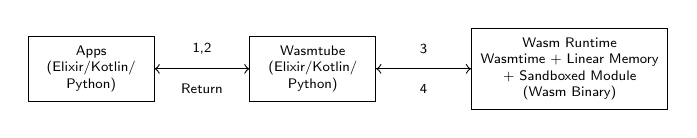
\begin{tikzpicture}[
    node distance=1.2cm,
    every node/.style={draw, minimum width=1.6cm, minimum height=0.5cm, align=center, font=\tiny}
]

% Nodes
\node (apps) {Apps \\ (Elixir/Kotlin/ \\ Python)};
\node (wasmtube) [right=of apps] {Wasmtube \\ (Elixir/Kotlin/ \\ Python)};
\node (runtime) [right=of wasmtube] {Wasm Runtime \\ Wasmtime + Linear Memory \\ + Sandboxed Module \\ (Wasm Binary)};

% Arrows with labels
\draw[->] (apps) -- node[above, font=\tiny, draw=none]
    {1,2} (wasmtube);

\draw[->] (wasmtube) -- node[above, font=\tiny, draw=none]
    {3} (runtime);

\draw[->] (runtime) -- node[below, font=\tiny, draw=none]
    {4} (wasmtube);

\draw[->] (wasmtube) -- node[below, font=\tiny, draw=none]
    {Return} (apps);

\end{tikzpicture}
}
\end{figure}

\textbf{Process Flow:}
\begin{enumerate}
\item \textbf{Initialization:} Host app starts Wasmtube with Wasm binary
\item \textbf{Function Calls:} Host app calls Wasmtube with function name and data
\item \textbf{Processing:} Wasm function processes data in sandboxed environment
\item \textbf{Response:} Results returned through Wasmtube to host app
\end{enumerate}

\end{frame}

% Slide 6: Wasmtube Bridge Architecture
\begin{frame}
\frametitle{Wasmtube: The Universal Wasm Bridge}
\framesubtitle{Enabling Cross-Language Communication with WebAssembly}

\textbf{Architecture and Functionality}

Wasmtube \cite{wasmtube2023} provides a simple API to instantiate Wasm sandboxes individualized for specific Wasm binaries. The library supports structured values and images as arguments to be passed into Wasm functions, enabling complex data exchange between Elixir applications and Wasm modules.

\textbf{Key Features:}
\begin{itemize}
\item \textbf{Language-Agnostic Design:} Same Wasm binary works all langs.
\item \textbf{Dynamic Updates:} Wasmtube can handle updates of Wasm binaries on-the-fly, allowing hot-swappable Wasm modules without system restart
\item \textbf{Structured Data Support:} Supports JSON-encoded structured values and binary-encoded images for complex data processing
\item \textbf{Linear Memory Management:} Efficient data exchange between host applications and Wasm modules through linear memory
\end{itemize}

\end{frame}



% Slide 7: Use Case: Machine Learning Inference
\begin{frame}
\frametitle{Use Case: Machine Learning Inference}
\framesubtitle{Isomorphic ML System Across IoT Layers}

\textbf{Deployment Architecture:}
\begin{itemize}
\item \textbf{Device Layer:} Raspberry Pi 4 (ARMv8-A)
\item \textbf{Edge Layer:} Google Cloud (x86/64)
\item \textbf{Local Layer:} iMac (arm64)
\end{itemize}

\textbf{ML Models Tested:}
\begin{itemize}
\item \textbf{ResNet-50:} 25M parameters, GPU-optimized (image classification)
\item \textbf{MobileNetV2:} Mobile-optimized, efficient (mobile inference)
\end{itemize}

\textbf{Process:} ONNX models $\rightarrow$ Apache TVM $\rightarrow$ Wasm binary $\rightarrow$ Deploy everywhere
\end{frame}

% Slide 9: Performance Results
\begin{frame}
\frametitle{Performance Results}
\framesubtitle{Quantitative Evaluation Results}

\textbf{Update Performance:}
\begin{itemize}
\item Traditional firmware: 10+ seconds
\item Wasm-based updates: 1.4 seconds
\item \textbf{Improvement:} 7x faster updates
\end{itemize}

\textbf{Function Call Overhead:}
\begin{itemize}
\item Native Elixir: 31.01 $\mu$s
\item Wasm function call: 252.48 $\mu$s
\item \textbf{Overhead:} $\sim$200 $\mu$s (acceptable for complex tasks)
\end{itemize}

\textbf{ML Inference Performance:}
\begin{itemize}
\item MobileNetV2 on Pi 4: 588.69 ms
\item MobileNetV2 on Cloud: 168.55 ms
\item MobileNetV2 on Local: 58.41 ms
\end{itemize}
\end{frame}

% Slide 10: Design Tradeoffs
\begin{frame}
\frametitle{Design Tradeoffs}
\framesubtitle{Technical Decisions and Tradeoffs}

\textbf{Tradeoff 1: Performance vs. Flexibility}
\begin{itemize}
\item \textbf{Cost:} 200$\mu$s overhead per Wasm call
\item \textbf{Benefit:} Dynamic updates without reboot
\item \textbf{Decision:} Acceptable for complex processing tasks
\end{itemize}

\textbf{Tradeoff 2: Portability vs. Hardware Acceleration}
\begin{itemize}
\item \textbf{Cost:} CPU-only execution (no GPU acceleration)
\item \textbf{Benefit:} Same binary across all platforms
\item \textbf{Future:} wasi-nn specification for GPU access
\end{itemize}

\textbf{Tradeoff 3: Simplicity vs. Functionality}
\begin{itemize}
\item \textbf{Cost:} Limited to Wasm-supported operations
\item \textbf{Benefit:} Simplified deployment and maintenance
\end{itemize}
\end{frame}

% Slide 9: Security and Privacy Considerations
\begin{frame}
\frametitle{Security and Privacy Considerations}
\framesubtitle{Security Implications of Wasm-Based IoT Systems}

\textbf{Security Benefits:}
\begin{itemize}
\item \textbf{Sandboxed Execution:} Wasm provides isolated execution environment
\item \textbf{Memory Safety:} Linear memory model prevents buffer overflows
\item \textbf{Code Integrity:} Binary verification before execution
\end{itemize}

\textbf{Security Challenges:}
\begin{itemize}
\item \textbf{System Interface Access:} Core application handles sensitive operations
\item \textbf{Update Security:} Need secure channels for Wasm binary distribution
\item \textbf{Runtime Security:} Wasm runtime must be kept updated
\end{itemize}

\textbf{Privacy Considerations:}
\begin{itemize}
\item \textbf{Data Processing:} ML models process sensitive image data
\item \textbf{Edge Processing:} Local inference reduces data transmission
\item \textbf{Compliance:} GDPR/privacy regulations for data handling
\end{itemize}
\end{frame}

% Slide 10: Outcomes and Impact
\begin{frame}
\frametitle{Outcomes and Impact}
\framesubtitle{Success Factors and Future Directions}

\textbf{Success Metrics:}
\begin{itemize}
\item $\checkmark$ \textbf{7x faster updates} compared to traditional methods
\item $\checkmark$ \textbf{Successful ML inference} across heterogeneous platforms
\item $\checkmark$ \textbf{Reduced development complexity} through code reuse
\item $\checkmark$ \textbf{Practical performance} suitable for real-world deployment
\end{itemize}

\textbf{Future Research Directions:}
\begin{enumerate}
\item \textbf{MLOps Integration:} Streamlined ML model deployment
\item \textbf{Workload Offloading:} Dynamic processing distribution
\item \textbf{Federated Learning:} Distributed ML training using Wasm
\end{enumerate}

\textbf{Industry Impact:} Enables rapid IoT development with reduced complexity
\end{frame}

% Slide 11: Summary
\begin{frame}
\frametitle{Summary}
\framesubtitle{Key Takeaways}

\textbf{Problem Solved:}
\begin{itemize}
\item Rapid IoT device updates without downtime
\item Simplified multi-platform IoT development
\end{itemize}

\textbf{Solution Delivered:}
\begin{itemize}
\item Dynamic IoT applications using WebAssembly
\item Isomorphic IoT systems with common codebase
\end{itemize}

\textbf{Results Achieved:}
\begin{itemize}
\item 7x faster update times
\item Successful cross-platform ML deployment
\item Practical performance characteristics
\end{itemize}

\textbf{Impact:} Demonstrates WebAssembly's potential to revolutionize IoT system development
\end{frame}

% Slide 12: References
\begin{frame}
\frametitle{References}
\framesubtitle{Sources and Additional Reading}

\textbf{Primary Reference:}
\begin{small}
K. Kuribayashi, Y. Miyake, K. Rikitake, K. Tanaka, and Y. Shinoda, ``Dynamic IoT Applications and Isomorphic IoT Systems Using WebAssembly,'' 2023 IEEE 9th World Forum on Internet of Things (WF-IoT), 2023.
\end{small}

\textbf{Key Technologies:}
\begin{itemize}
\item WebAssembly: \url{https://webassembly.org/}
\item Apache TVM: \url{https://tvm.apache.org/}
\item Nerves Platform: \url{https://nerves-project.org/}
\item Wasmtime Runtime: \url{https://wasmtime.dev/}
\end{itemize}

\textbf{Related Work:}
\begin{small}
S. Bansal and D. Kumar, ``IoT ecosystem: A survey on devices, gateways, operating systems, middleware and communication,'' Int. J. Wireless Inf. Networks, 2020.
\end{small}

\textbf{Questions?}
\end{frame}

\end{document}
